\documentclass[a4paper, twoside]{report}

\usepackage[english]{babel}
\usepackage[utf8]{inputenc}
\usepackage[T1]{fontenc}
\usepackage{listings}
\usepackage{hyperref}
\hypersetup{hidelinks}
\usepackage{lscape}
\usepackage{amsmath}
\usepackage{graphicx}
\usepackage[colorinlistoftodos]{todonotes}
\usepackage[
    backend=biber,
    style=numeric,
		sorting=none,
    natbib=true,
    url=false,
    doi=true,
    eprint=false
]{biblatex}
\addbibresource{bibs/sample.bib}

% \usepackage{caption}
\usepackage{subcaption}
% \usepackage{xcolor}
\usepackage{makeidx}
\definecolor{dkgreen}{rgb}{0,0.6,0}
\definecolor{gray}{rgb}{0.5,0.5,0.5}
\definecolor{mauve}{rgb}{0.58,0,0.82}
\usepackage{tikz}
\usetikzlibrary{arrows}
\usepackage{verbatim}
\usepackage{bm}
\usepackage{float}
\usepackage{mathpazo} % Palatino font
\usepackage[a4paper,top=3cm,bottom=4cm,left=3cm,right=3cm,marginparwidth=1.75cm]{geometry}
\usepackage[edges]{forest}
\definecolor{foldercolor}{RGB}{124,166,198}
\tikzset{pics/folder/.style={code={%
		\node[inner sep=0pt, minimum size=#1](-foldericon){};
		\node[folder style, inner sep=0pt, minimum width=0.3*#1, minimum height=0.6*#1, above right, xshift=0.05*#1] at (-foldericon.west){};
		\node[folder style, inner sep=0pt, minimum size=#1] at (-foldericon.center){};}
		},
		pics/folder/.default={20pt},
		folder style/.style={draw=foldercolor!80!black,top color=foldercolor!40,bottom color=foldercolor}
}

\forestset{is file/.style={edge path'/.expanded={%
		([xshift=\forestregister{folder indent}]!u.parent anchor) |- (.child anchor)},
		inner sep=1pt},
		this folder size/.style={edge path'/.expanded={%
		([xshift=\forestregister{folder indent}]!u.parent anchor) |- (.child anchor) pic[solid]{folder=#1}}, inner xsep=0.6*#1},
		folder tree indent/.style={before computing xy={l=#1}},
		folder icons/.style={folder, this folder size=#1, folder tree indent=3*#1},
		folder icons/.default={12pt},
}
\renewcommand{\baselinestretch}{1.3}
\lstset{frame=tb,
  language=Matlab,
  aboveskip=3mm,
  belowskip=3mm,
  showstringspaces=false,
  columns=flexible,
  basicstyle={\small\ttfamily},
  numbers=none,
  numberstyle=\tiny\color{gray},
  keywordstyle=\color{blue},
  commentstyle=\color{dkgreen},
  stringstyle=\color{mauve},
  breaklines=true,
  breakatwhitespace=true,
  tabsize=3
}

\title{Structure and dynamics of large networks of interacting neurons}
\author{Alejandro Gilson Campillo}
% Update supervisor and other title stuff in title/title.tex

\begin{document}
\begin{titlepage}

\newcommand{\HRule}{\rule{\linewidth}{0.5mm}} % Defines a new command for the horizontal lines, change thickness here

%----------------------------------------------------------------------------------------

\center % Center everything on the page

%----------------------------------------------------------------------------------------
%	HEADING SECTIONS
%----------------------------------------------------------------------------------------
\quad\\[1.5cm]
%\textsc{\LARGE MSc Thesis}\\[1.5cm] % Name of your university/college
\textsc{\Large Imperial College London}\\[0.5cm] % Major heading such as course name
\textsc{\large Department of Electrical and Electronic Engineering}\\[0.5cm] % Minor heading such as course title

%----------------------------------------------------------------------------------------
%	TITLE SECTION
%----------------------------------------------------------------------------------------
\makeatletter
\HRule \\[0.4cm]
{ \huge \bfseries \@title}\\[0.4cm] % Title of your document
\HRule \\[1.5cm]
 
%----------------------------------------------------------------------------------------
%	AUTHOR SECTION
%----------------------------------------------------------------------------------------

\begin{minipage}{0.4\textwidth}
\begin{flushleft} \large
\emph{Author:}\\
\@author\\ % Your name
\emph{CID:}\\
01112712\\
\end{flushleft}
\end{minipage}
~
\begin{minipage}{0.4\textwidth}
\begin{flushright} \large
\emph{Supervisor:} \\
Dr. Pier Luigi Dragotti \\
\emph{Second marker:} \\
Dr. Wei Dai
% Uncomment the following lines if there's a co-supervisor
%\\[1.2em] % Supervisor's Name
%\emph{Co-Supervisor:} \\
%Dr. Adam Smith % second marker's name
\end{flushright}
\end{minipage}\\[3cm]
\makeatother

%	LOGO SECTION
%----------------------------------------------------------------------------------------


\includegraphics[width=4cm]{title/imperialcollegelondon.jpg}\\[1cm] % Include a department/university logo - this will require the graphicx package
 
%----------------------------------------------------------------------------------------

%----------------------------------------------------------------------------------------
%	DATE SECTION
%----------------------------------------------------------------------------------------

{\large A thesis submitted for the degree of}\\[0.5cm]
{\large \emph{MEng Electrical and Electronic Engineering}}\\[0.5cm]
{\large \today}\\[2cm] % Date, change the \today to a set date if you want to be precise

\vfill % Fill the rest of the page with whitespace

\end{titlepage}


\begin{abstract}
This project tries to understand how real biological neural networks are connected by treating the system as a diffusion process. By selecting the connectivity weights of each of the neurons that maximize the likelihood of some recorded spikes occurring  the structure of the network is estimated. For this project, the speed and scalability of NetRate (the implemented algorithm) is improved and its constraints are analysed. Moreover, the model of neural network and inference algorithm are changed for it to be used on a real mouse’s spike data-set and a benchmark is presented for analysing inference accuracy when no ground truth is available.
\end{abstract}

\renewcommand{\abstractname}{Acknowledgements}
\begin{abstract}
It is usual to thank those individuals who have provided particularly useful assistance, technical or otherwise, during your project.
\end{abstract}

\tableofcontents
\listoffigures
\listoftables


\chapter{Introduction}

The brain is a complex machine, it allows the human being to think, communicate and feel. It does so thanks to the billions of neurons that communicate in a dense network through synapses. However, little is known about how it works. By studying how the neurons structure to store and process information we can understand how the brain as a whole functions. This could have important applications in medicine for curing diseases such as Parkinson \cite{OldeDubbelinkKimT.E.2014Dbnt} and epilepsy \cite{PONTEN2007918}, and in machine learning for the development of more intelligent neural networks.\\

In order to infer the network structure of a set of neurons, they are treated as a diffusion network where electrical spikes increase the likelihood of connected neurons to spike and therefore transmit a signal that travels as if it were a disease. By evaluating the time of "infection", the relationship between two neurons can be probabilistically estimated. After computing the relationship between all of the neurons, an estimate of the topology of the network can be obtained. \\

Previous work on this topic \cite{pranav_report, alexandru2018estimating} evaluated the feasibility of using a maximum-likelihood estimator algorithm, NetRate \cite{rodriguez2011uncovering}, for the inference of the structure of biological neural networks. A network was simulated using the Izhikevic neuron model \cite{izhikevich2003simple} and the Brian simulator \cite{10.3389/neuro.01.026.2009}. The connections between the neurons were then estimated, compared to the original network and the performance of the algorithm was evaluated. Recent developments in technology now allow scientists to obtain individual neuron spike information from the brain tissue \cite{ito2016spontaneous, ito2014large, litke2004does}. This data is very useful and serves as a mean of evaluating the performance of the algorithm with real neurons. Moreover, this information can help in creating simulated networks that resemble more the real biological ones.




\graphicspath{ {background/} }
\chapter{Background}

\section{Definition of connectivity}

The definition of connectivity between neurons has a history of lack of consensus among the scientific community. Connectivity studies from different researchers may lead to different results depending on how they define it, as they may be looking at different aspects of connectivity. The two main accepted definitions that are used are functional and effective connectivity \cite{HORWITZ2003466}.
\\\\
Functional connectivity is the temporal correlation between spatially remote neurophysiological events \cite{friston1993functional}. Studies on this topic began with electroencephalography (EEG) measurements. Some methods to measure functional connectivity include the evaluation of the correlation in the frequency domain between EEG signals at different scalp locations \cite{pfurtscheller1999event}, and the cross-correlation of the time series measurements from a pair of electrodes \cite{gevins1985neurocognitive}. However, due to the volume conduction of brain tissue, the electrical activity from the scalp cannot infer the individual neuron behaviour below the electrode \cite{HORWITZ2003466}.
\\\\
Effective connectivity was defined in \cite{friston1993functional} as the influence that one neural system exerts on another. Effective connectivity can be measured in terms of efficacy and contribution. At a synaptic level it can be expressed as in Eq.\ref{eq:synaptic_effectivity}, where $x_{j}$ is the post-synaptic response to many pre-synaptic inputs $x_{i}$ and $\textbf{W}_{ij}$ is the efficacy of the connections between neurons $i$ and $j$. Contribution is reflected in Eq.\ref{eq:synaptic_contribution} as the effect of $i$ on $j$ relative to all pre-synaptic inputs. Using this definition, directional effects are taken into account and a richer representation of the network can be attained. Following the approach in \cite{alexandru2018estimating}, this project will focus on the effective connectivity of neurons in a network.
\\

\begin{equation}\label{eq:synaptic_effectivity}
x_{j} = \Sigma \textbf{W}_{ij}\times x_{i}
\end{equation}

\begin{equation}\label{eq:synaptic_contribution}
\frac{\textbf{W}_{ij}}{\Sigma \textbf{W}_{ij}}
\end{equation}

\section{Izhikevich neuron model}\label{sec:izhikevich_neuron_model}

In order to understand how the brain works we must be able to replicate the behaviour of individual neurons applying simple and accurate models. However, as explained in \cite{izhikevich2003simple}, meeting both criteria can be challenging. The Hodgkin–Huxley model \cite{hodgkin1952quantitative} is very accurate as it can emulate the rich firing patterns of many types of neurons. However, it is very computationally expensive and only a few neurons can be computed in real time. The integrate-and-fire model \cite{burkitt2006review}  has the opposite problem: it is computationally simple but it is an unrealistic representation of the neuron since it does not capture the firing patterns with sufficient accuracy \cite{izhikevich2003simple}. In contrast, the Izhikevich neuron model \cite{izhikevich2003simple} meets both criteria. Tens of thousands of spiking cortical neurons can be simulated in real time by simplifying the Hodgkin-Huxley model into the two dimensional system of differential equations shown below.


\begin{align}\label{eq:izhikevich_ode}
&v'=0.04v^{2}+5v+140-u+I \\
&u'=a(bv-u)
\end{align}

with the auxiliary after-spike reseting

\begin{equation}\label{eq:izhikevich_reset}
\text{if } v \geq 30 \text{mV, then}
\begin{cases}
    v     & \leftarrow c \\
    u     & \leftarrow u + d 
  \end{cases}
\end{equation}

Here, the dimensionless variables $v$ and $u$ represent the membrane potential of the neuron and the membrane recovery, respectively. When a spike reaches its apex (30 mV), both these variables are reset according to Eq. \ref{eq:izhikevich_reset}. The differentiation is taken with respect to time. Synaptic or injected DC currents are represented by the variable $I$. Just as with real neurons, the threshold is not fixed and it's based on previous spikes. 
\\
On the other hand, $a, b, c$ and $d$ are dimensionless parameters. $a$ determines the speed of the recovery variable $u$, $b$ defines the sensitivity of the recovery variable $u$ to sub-threshold fluctuations of the membrane potential $v$. Finally, $c$ and $d$ determine the after-spike reset value of the recovery variables $v$ and $u$, respectively. 
\\\\
The relevance of this algorithm stems from the fact that, different combinations of the parameters provide the model with a rich variety of firing patterns. When analysing the neocortical neurons in the mammalian brain, a number of different classes of excitatory neurons can be found \cite{connors1990intrinsic, gray1996chattering} such as RS (regular spiking), IB (intrinsically bursting) and CH (chattering). From the inhibitory type of neurons, two classes can be found: FS (fast spiking and LTS (low-threshold spiking). Other interesting classes of neurons are the TC (thalamo-cortical) and the RZ (resonator). A visual representation of these neurons can be observed in figure \ref{fig:types_neurons}. It is of great importance to understand what types of neurons can be found so that a simulated network can become a closer representation of what can be found on a real brain. In order to simplify the network to be inferred, the only type of neurons simulated in the network were the excitatory regular spiking neurons. This was achieved by setting the parameters to $a=0.02$, $b=0.2$, $c=-65$ and $d=8$. This type of neuron is the most common type of excitatory neuron in the brain. There is also a ratio of excitatory and inhibitory neurons of 4 to 1 in the mammalian brain, respectively \cite{izhikevich2003simple}.

In order to make use of the Izhikevich neuron model, Eq.\ref{eq:izhikevich_ode} is input to the Brian Simulator. This library computes the membrane potential voltage of the interacting neurons in the network and outputs all of their spiking times. This data will then be used to compute the NetRate algorithm.


\begin{figure}
  \centering
	\begin{subfigure}[b]{0.49\textwidth}
		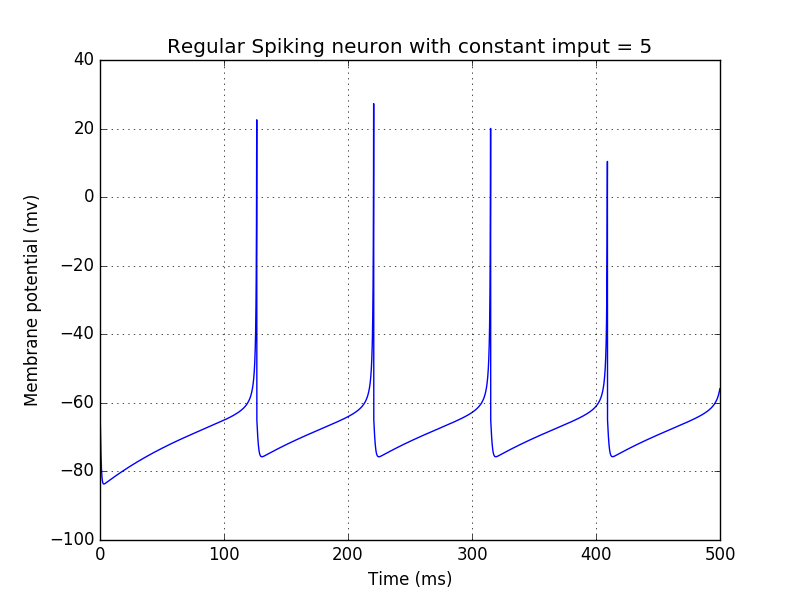
\includegraphics[width=\textwidth]{regular_spiking.png}
	\end{subfigure}
	\begin{subfigure}[b]{0.49\textwidth}
		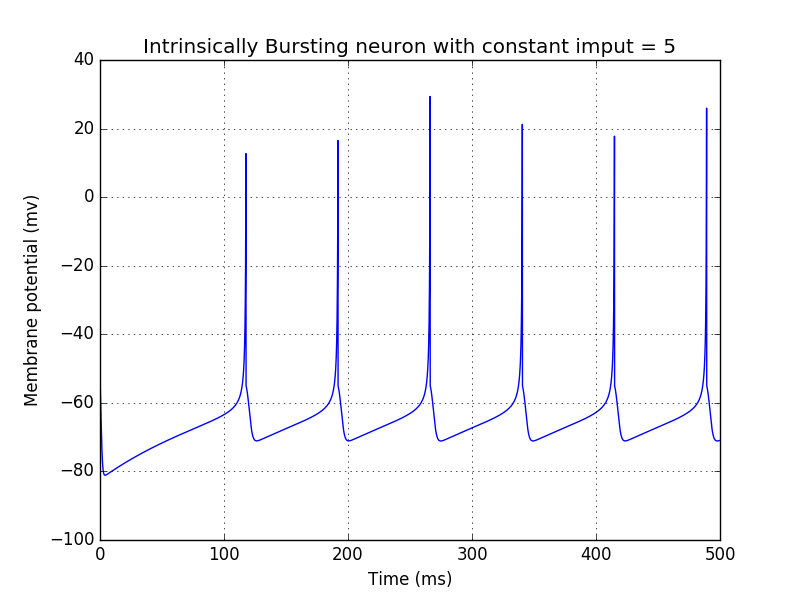
\includegraphics[width=\textwidth]{intrinsically_bursting.png}
	\end{subfigure}
	\begin{subfigure}[b]{0.49\textwidth}
		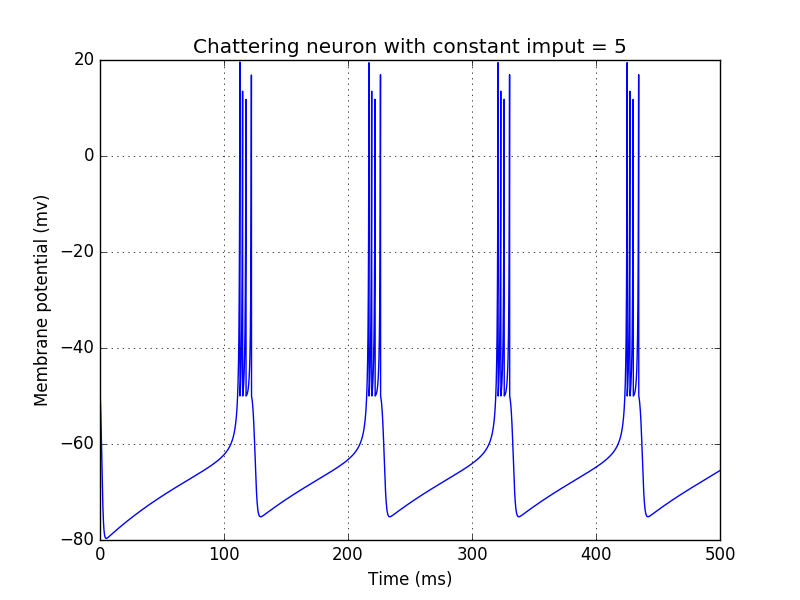
\includegraphics[width=\textwidth]{chattering.png}
	\end{subfigure}
	\begin{subfigure}[b]{0.49\textwidth}
		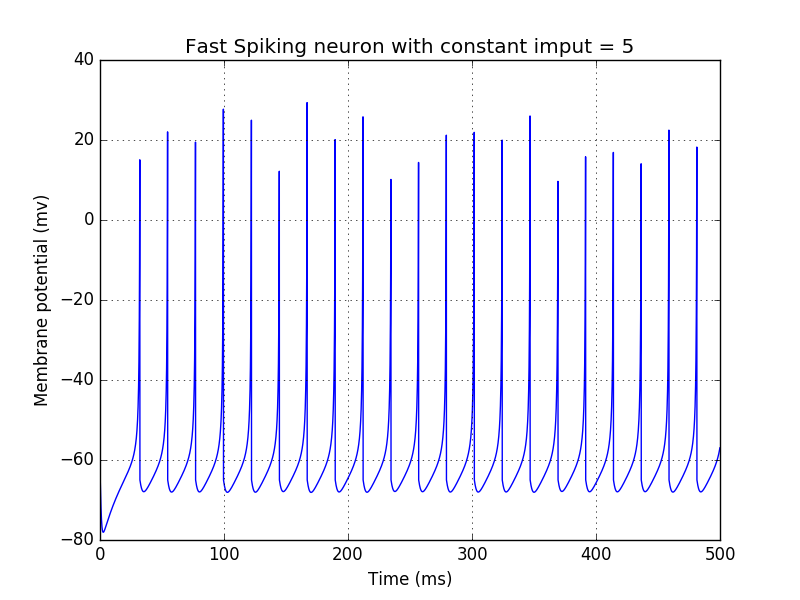
\includegraphics[width=\textwidth]{fast_spiking.png}
	\end{subfigure}
  \caption{Types of neurons in the mammalian brain. Generated with the Brian Simulator \cite{10.3389/neuro.01.026.2009} using the Izhikevich neuron model \cite{izhikevich2003simple}}
	\label{fig:types_neurons}
\end{figure}


\section{Netrate}

\subsection{Diffusion processes}\label{sec:diffusion_processes}

In order to infer the underlying structure of a network, \cite{alexandru2018estimating} employed the NetRate algorithm developed by Rodriguez \cite{rodriguez2011uncovering} by treating the network as a diffusion process.

The study of diffusion networks is based on the observation of the nodes in a system when they take a certain action: get infected by a virus, share a piece of information, etc. A problem concerning this kind of studies lies on the fact that we can only understand when and where these nodes propagate but not how or why the do so. An example of this is the propagation of a virus in a population. We can tell who and when somebody got infected but not who infected him. For the rest of this section we will refer to the propagation of an infection as the object of study of the network. 

To infer the mechanisms behind diffusion processes the time of infection is analysed. A model needs to be created with some assumptions about the structures that generate diffusion processes:

\begin{itemize}
\item The network in a diffusion process is fixed, unknown and directed: Connections do not change in time, it is not known what the connections are and connections are not bilateral.
\item Infections are binary, they can only be infected or not infected, no partial infections are considered. For real neurons this means that there is either a spike or there is not.
\item Infections across the edges of the network occur independently from one another. The probability of node $i$ being infected by node $j$ is not dependent on what the probability of node $k$ infecting node $i$ is.
\item The likelihood of a node $a$ infecting node $b$ at time $t$ is modelled by a probability distribution dependent on $a, b$ and $t$.
\item All infections in a network are observed during a recorded time window. This time frame is called horizon \cite{rodriguez2011uncovering}. The larger the horizon, the higher the probability of more infections.
\end{itemize}

NetRate aims to describe how infections occur during a period of time in a fixed network. This is achieved by finding the optimal network and transmission rates that maximize the likelihood of a set of observed cascades to occur. The mathematical definitions that construct this model will be explained in the following section.


\subsection{Mathematical definitions}

The following definitions in this section are necessary for the construction of the model with which we intend to infer the connectivity of the network. First, the data that is going to be analysed will be defined:
\\\\
Observations are carried out on a population of $N$ nodes that have created a set of $C$ cascades $\{\textbf{t}^{1},\cdots,\textbf{t}^{|C|}\}$. Each of the cascades $\textbf{t}^{c}$ contains the infection times of all the population within a time period $T^{c}$. Each of these cascades is an N-dimensional vector with recordings of when the nodes were infected in the cascade. If a node was not infected during the time period $[0,T^{c}]$, a symbol $\infty$ is assigned. This does not mean that the node never gets infected. For simplicity, we define $T^{c}=T$. Node $i$ is parent of node $j$ if $t_{i}<t_{j}$ within the cascade.


\begin{equation}\label{eq:data_netrate}
\textbf{t}^{c}:=(t_{1}^{c},\cdots,t_{N}^{c}),\quad t_{k}^{c}\in [0,T^{c}]\cup{\infty}
\end{equation}

The pairwise interactions are to be studied in order to obtain the pairwise transmission likelihood between nodes in the network. It will be assumed that infections can occur at different rates along different edges in the network. 

\begin{itemize}
\item $f(t_{i}|t_{j},\alpha _{j,i})$ is the conditional likelihood of transmission between nodes $j$ and $i$. It depends on the infection times $(t_{i},t{j})$ and pairwise transmission rate $\alpha_{j,i}$.
\item A node cannot be infected by a healthy node. Node $j$, infected at $t_{j}$, can only infect node $i$ at time $t_{i}$ if and only if $t_{j}<t_{i}$.
\item Transmission rate $\alpha _{j,i}\geq0$.
\end{itemize}

The cumulative density function is defined as $F(t_{i}|t_{j};\alpha _{j,i})$ and is obtained from the transmission likelihood. If a node $j$ was infected at time $t_{j}$, the probability that node $i$ is not infected by node $j$ by time $t_{i}$ is given by the survival function of the edge $j\rightarrow i$:

\begin{equation}\label{eq:survival_function}
S(t_{i}|t_{j};\alpha _{j,i})=1-F(t_{i}|t_{j};\alpha _{j,i})
\end{equation}

The instantaneous infection rate, or hazard function, of the edge $j\rightarrow i$ is the ratio of the transmission likelihood over the survival function as shown in Eq.\ref{eq:hazard_function}.

\begin{equation}\label{eq:hazard_function}
H(t_{i}|t_{j};\alpha _{j,i})=\frac{f(t_{i}|t_{j};\alpha _{j,i})}{S(t_{i}|t_{j};\alpha _{j,i})}
\end{equation}

With a complete set of definitions, it will now be possible to derive the algorithm behind NetRate as it will be shown in the next section.

\subsection{Derivation of NetRate}

Rodriguez \cite{rodriguez2011uncovering} derives NetRate by studying the individual probability of infection of the nodes and then building the whole of the network. The probability of survival of any cascade is the probability that a node is not infected until time $T$, given that the parents are infected at the beginning of the cascade. For a non-infected node $i$, the probability that any of the nodes $1\cdots N$ does not infect node $i$ by time $T$ is given by the product of the survival functions of each of the infected nodes $k$ targeting node $i$ because the different probabilities of infection are considered independent. This is illustrated in Eq.\ref{eq:step_1_netrate}.

\begin{equation}\label{eq:step_1_netrate}
\prod_{t_{k}\leq T}S(T\mid t_{k};\alpha _{k,i})
\end{equation}

To compute the likelihood of a cascade $\textbf{t}:=(t_{1},\cdots,t_{N}|t_{i}\leq T)$ we require the the likelihood of the recorded infections $\textbf{t}^{\leq T}=(t_{1},\cdots,t_{N}|t_{i}\leq T)$. Again, using independence, the likelihood factorizes as seen in \ref{eq:step_2_netrate}. The likelihood of the cascade then becomes the conditional likelihood of the infection time given the rest of the cascade.

\begin{equation}\label{eq:step_2_netrate}
f(\textbf{t}^{\leq T};\textbf{A})=\prod_{t_{i}\leq T}f(t_{i}\mid t_{1},\cdots,t_{N}\backslash t_{i};\textbf{A})
\end{equation}

As in \cite{kempe2003maximizing}, a node gets infected when the first parent infects the node. We now compute the likelihood of a potential parent $j$ of being the first one by using Eq.\ref{eq:step_1_netrate}.

\begin{equation}\label{eq:step_3_netrate}
f(t_{i}\mid t_{j};\alpha_{j,i})\times \prod_{j\neq k,t_{k}< t_{i}}S(t_{i}\mid t_{k};\alpha _{k,i})
\end{equation}
 
In this step, we calculate the conditional likelihood of Eq.\ref{eq:step_2_netrate} by adding all the likelihoods of the mutually disjoint likelihoods that each potential parent is the first parent:

\begin{equation}\label{eq:step_4_netrate}
f(t_{i}\mid t_{1},\cdots,t_{N}\backslash t_{i};\textbf{A})=\sum_{j:t_{j}<t_{i}}f(t_{i}\mid t_{j};\alpha _{j,i})\times \prod _{j\neq k,t_{k}<t_{i}}S(t_{i}\mid t_{k};\alpha _{k,i})
\end{equation}

Using Eq.\ref{eq:step_2_netrate} and removing the condition $k\neq j$, the likelihood of infections then becomes:

\begin{equation}\label{eq:step_5_netrate}
f(\textbf{t}^{\leq T};\textbf{A})=\prod_{t_{i}\leq T}\prod_{k:t_{k}<t_{i}}S(t_{i}\mid t_{k};\alpha _{k,i})\times \sum_{j:t_{j}<t_{i}}\frac{f(t_{i}\mid t_{j};\alpha_{j,i})}{S(t_{i}\mid t_{j};\alpha _{j,i})}
\end{equation}

However, Eq.\ref{eq:step_5_netrate} needs to consider also the nodes that are not infected during the observation window. For this reason we add the multiplicative survival term from Eq.\ref{eq:step_1_netrate} and replace the ratios from Eq.\ref{eq:step_5_netrate} with hazard functions:

\begin{equation}\label{eq:step_6_netrate}
f(\textbf{t};\textbf{A})=\prod_{t_{i}\leq T}\prod_{t_{m}>T}S(T\mid t_{i};\alpha_{i,m})\times \prod_{k:t_{k}<t_{i}}S(t_{i}\mid t_{k};\alpha _{k,i})\sum_{j:t_{j}<t_{i}}H(t_{i}\mid t_{j};\alpha _{j,i})
\end{equation}

The likelihood of a set of independent set of cascades $C=\{t^{1},\cdots,t^{|C|}\}$ is the product of the likelihoods of all the individual cascades given by Eq.\ref{eq:step_6_netrate}:

\begin{equation}\label{eq:step_7_netrate}
\prod _{\textbf{t}^{c}\in C}f(\textbf{t}^{c};\textbf{A})
\end{equation}

The goal of the algorithm is to find the transmission rates $\alpha_{j,i}$ of all the edges in the network such that the likelihood of the set of cascades is maximized.

\begin{subequations}
\label{eq:optimization_netrate}
\begin{align}
& \text{minimize}_{\textbf{A}} -\sum_{c\in C}\log f(\textbf{t};\textbf{A})\\
& \text{subject to } \alpha _{j,i}\geq 0,i,j=1,\cdots,N,i\neq j,
\end{align}
\end{subequations}.

Here, $\textbf{A}:=\{\alpha _{j,i}\mid i,j=1,\cdots,n,i\neq j\}$ are the variables and the edges of the network are defined as the pairs of nodes whose transmission rates $\alpha _{i,j}>0$. 
\\\\
The solution to Eq.\ref{eq:optimization_netrate} found in \cite{rodriguez2011uncovering} is given by Eq.\ref{eq:solution_netrate}. The survival and hazard functions are concave in the parameter(s) of the transmission likelihoods and, therefore, convexity of Eq.\ref{eq:optimization_netrate} follows from linearity. The network inference problem from Eq.\ref{eq:optimization_netrate} is thus convex for Power-Law, Rayleigh and Exponential models of the likelihood function.

\begin{subequations}
\begin{align}
\label{eq:solution_netrate}
& L(\{\textbf{t}^{1}\cdots \textbf{t}^{|C|}\};\textbf{A})=\sum _{c}\Psi_{1}(\textbf{t}^{c};\textbf{A})+\Psi_{2}(\textbf{t}^{c};\textbf{A})+\Psi_{3}(\textbf{t}^{c};\textbf{A})\\
& \Psi_{1}(\textbf{t}^{c};\textbf{A})=\sum _{i:t_{i}\leq T}\sum _{t_{m}>T}\log S(T\mid t_{i};\alpha _{i,m})\\
& \Psi _{2}(\textbf{t}^{c};\textbf{A})=\sum_{i:t_{i}\leq T} \sum_ {j:t_{j}<t_{i}}\log S(t_{i}\mid t_{j};\alpha_{j,i})\\
& \Psi _{3}(\textbf{t}^{c};\textbf{A})=\sum_{i:t_{i}\leq T} \log (\sum_{j:t_{j}<t_{i}} H(t_{i}\mid t_{j};\alpha_{j,i}))
\end{align}
\end{subequations}

The terms in Eq.\ref{eq:solution_netrate} depend only on the infection time differences ($t_{i}-t_{j}$) and the transmission rates $\alpha_{j,i}$. Each of the terms adds a property to the solution of NetRate.

\begin{itemize}
\item The terms $\Psi_{1}$ and $\Psi_{2}$ apply a positively weighted norm on $\textbf{A}$, thus encouraging sparse solutions.
\item $\Psi_{2}$ penalizes the edges that transmit infections slowly and promotes edges that infect quickly.
\item $\Psi_{1}$ penalizes edges to uninfected nodes until the time horizon. With a longer observation window the penalties become larger, but so does the probability of nodes becoming infected.
\item $\Psi_{3}$ makes sure that all infected nodes have a minimum of one parent to avoid $\log 0 = -\infty$. Since the logarithm grows slowly, it slightly encourages infected nodes to have many parents.
\end{itemize}

\subsection{Cascade generation}\label{sec:cascade_generation}

The maximization of the likelihood function requires data in the form of cascades in order to be computed. The time of infection of each of the nodes can be obtained from the network simulation but it must then be formatted into cascades. The rest of this section is based on \cite{pranav_report}, where cascade generation is explained. 

\begin{enumerate}
\item At time $t=0$, a random node is selected to carry the disease.
\item The disease propagates for a $T$ amount of time (horizon) based on the pairwise transmission likelihood $f(t_{i}\mid t_{j};\alpha_{j,i})$ of the edges in the network.
\item At the end of the simulation, a cascade is generated with the information from the times at which the nodes were infected. 
\end{enumerate}

As an example, let there be a network of 6 nodes ($N=6$) and a horizon of $T=20$. Let us select node 5 at time $t=0$ to be the starting point of the experiment. The simulation begins and the disease spreads out. It infects node 2 at $t=3$ and node 6 at $t=5$. The resulting cascade has the form of Eq.\ref{eq:data_netrate}  would look like this:

\begin{equation}\label{eq:cascade_example}
\textbf{t}^{c}=\{\infty, 3, \infty, \infty, 0, 5\}
\end{equation}

Remember from Eq.\ref{eq:data_netrate} that the symbol $\infty $ represents a node that is not infected during the cascade. Nodes 2 and 6 were infected while nodes 1, 3 and 4 remained healthy for the duration of the cascade. Since at time $t=3$ the only infected node was 3, this node must have infected node 2. However, it becomes inconclusive as to which node infected 6 at time $t=6$. We could be lead to believe that the uninfected nodes are not connected to any of the other infected nodes. However, cascades are probabilistic models and no one cascade can tell us what the values of $\alpha_{j,i}$ are. We would, therefore, require a large number of cascades in order to infer those values with a high confidence. 


\subsection{Performance metrics}\label{sec:performance_metrics}

Evaluating the performance of NetRate involves analysing the inferred network $\hat G$: which edges have been correctly inferred, which ones have been missed and what weights have been assigned to the inferred edges. These questions are answered in \cite{rodriguez2011uncovering} by calculating the accuracy, precision, recall and MAE against the true network $G^{*}$:

\begin{enumerate}
\item Precision is the proportion of edges in the inferred network that exist in the true network.
\item Recall is the proportion of edges in the true network that exist in the inferred network.
\item $\text{Accuracy}=1-\frac{\sum_{i,j}\mid I(\alpha_{i,j}^{*})-I(\hat \alpha_{i,j}\mid}{\sum_{i,j}I(\alpha^{*}_{i,j})+\sum_{i,j}I(\hat \alpha _{i,j})}, \quad \text{where } I(\alpha)=1\text{ if } \alpha > 0\text{ and } I(\alpha)=0\text{, otherwise.}$
\item $\text{MAE} = E[\mid \alpha^{*} - \hat \alpha \mid /\alpha^{*}], \quad $ where $ \alpha^{*}$ and $\hat \alpha $ are the true and estimated transmission rates, respectively.
\end{enumerate}

\section{Biological Neural Network}

\subsection{Structure of the Network}

In order to understand how neural networks are connected, a clear visual representation is required. This is achieved with an adjacency matrix plot. These matrices can be of three different types: binary ($\alpha_{i,j}\in\{0,1\}$), ternary ($\alpha_{i,j}\in\{-1,0,1\}$) or real ($\alpha_{i,j}\in \mathbb{R}$). Due to the characteristics of biological neuron connections, real adjacency matrices are employed. In figure \ref{fig:graph_20_nodes} an adjacency matrix of a network of 20 nodes can be observed. When $\alpha_{j,i}^{BNN}\neq 0$, the target neuron $i$ and the source neuron $j$ are connected and a dot appears on the graph. The source nodes are indexed in the x-axis and the target nodes on the y-axis. The weight of each of the edges is represented by the diameter of the dot. \\

\begin{figure}
  \centering
  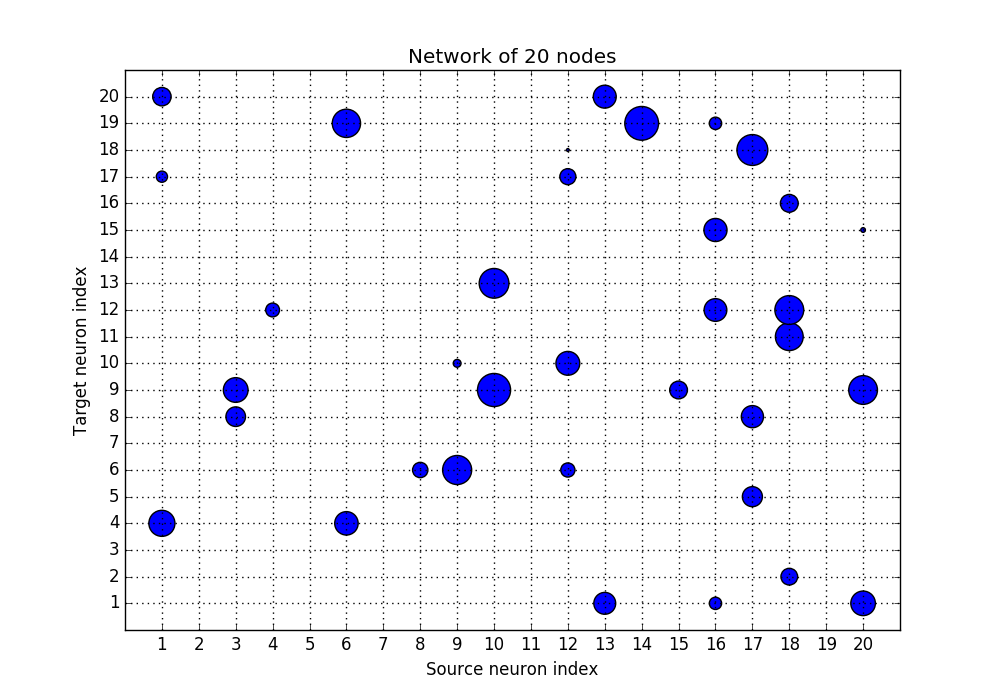
\includegraphics[width=0.8\textwidth]{graph_20_nodes.png}
	\label{fig:graph_20_nodes}
  \caption{Adjacency matrix of a network of 20 nodes}
\end{figure}

The superscript \textit{BNN} in $\alpha_{j,i}^{BNN}$ is employed to differentitate between the weights in biological neural networks and the analogous transmission rates $\alpha_{j,i}$ in diffusion networks \cite{pranav_report}. When neurons $j$ and $i$ are connected with a weight $\alpha_{j,i}^{BNN}$, everytime $j$ spikes, it causes the membrane potential $v$ from Eq.\ref{eq:izhikevich_ode} to increase by $\alpha_{j,i}^{BNN}$. If neuron $i$ crosses the threshold of 30mV, it spikes. This phenomenon is proved in \cite{alexandru2018estimating} and explained in section \ref{sec:input_stimulus_model_for_cascade_generation}. Using the example in figure \ref{fig:graph_20_nodes}, when node 10 spikes, it causes nodes 13 and 9 to increase by $\alpha_{10,13}^{BNN}$ and $\alpha_{10,9}^{BNN}$, respectively. 

The type of networks that were simulated in \cite{alexandru2018estimating} are generated by Erdös \& Reny random graphs, where each possible edge in the network has an independent probability $p$ of being present. The weights assigned to the edges are the output of a uniform distribution in (0,30], the threshold value in Eq.\ref{eq:izhikevich_ode}. It can be observed that the adjacency matrix does not contain weights where $i=j$ because spikes do not increase the membrane potential of the source neuron.


\subsection{Input stimulus model for cascade generation}\label{sec:input_stimulus_model_for_cascade_generation}

The neurons in the brain are susceptible to input stimuli from the rest of the neurons in the network. This is represented in the Izhikevich neuron model with the $I$ component in Eq.\ref{eq:izhikevich_ode}. This term can be employed to model injected current in the form of a DC input or can be normally distributed\footnote{In the Izhikevich neuron model \cite{izhikevich2003simple}, the mean and standard deviation are equal to 0 and 5 for excitatory neurons and to 0 and 2 for inhibitory neurons, respectively.} to represent noise from interactions with neurons that are outside the network being recorded.\\

The selection of an appropriate input stimulus for the neurons was a challenge encountered by Malhotra \cite{alexandru2018estimating}. With a Gaussian input $I$, neurons spike at random times and there is no systematic way of selecting the beginning of a cascade. In a cascade where nodes 1, 3 and 5 spike in chronological order, each of them could have in turn their own cascade (i.e 1, 3 and 5; 3 and 5; and 5). However, this breaks the requirement of independence of cascades seen in section \ref{sec:diffusion_processes}, where no same spike can appear in two cascades. For this reason, a well studied approach was required for the selection of cascades. 

The solution Malhotra found to this problem was to provide one neuron at a time with a constant input of 12mV and the rest of the neurons with Gaussian noise. This caused the selected neuron to spike periodically. With an appropriate selection of the DC input, the spiking frequency could be changed, and with a sufficiently long time between spikes, the network could settle into a steady state. Unlike infections in diffusion networks, neurons can spike more than once. For this reason the horizon was arbitrarily limited so as to not allow two spikes from the same cascade to occur in the same cascade and, therefore, obey the law of binary infections imposed by NetRate \cite{alexandru2018estimating}.\\

This method provides a systematic way of generating cascades: every time the node with DC input spiked, a new independent cascade was created. In order to obtain cascade information from all the nodes in the network, all nodes are stimulated over the course of an experiment. Otherwise, if only one node was selected, no information would be extracted from the nodes with no direct connection to it \cite{pranav_report}. \\

The experimental results obtained by Malhotra show that an optimal amount of spiking information that achieves a high inferring performance is achieved with a stimulation time of 4,000 ms. This is due to the underlying probabilistic nature of NetRate \cite{pranav_report}. In other words, more data does not result in a higher performance.

\subsection{Likelihood function}

The ability of NetRate to infer the weights in the adjacency matrix \textbf{A} stems from the fact that the shape of $f(t_{i}\mid t_{j};a_{j,i})$ provides a probabilistic description of $\alpha_{j,i}$. The Izhikevich spiking neuron is modelled deterministically while the propagation of infections is probabilistic. For this reason the suitability of NetRate for the biological network inference was proved in \cite{alexandru2018estimating}.\\

As was explained in section \ref{sec:cascade_generation}, it is not possible to determine exactly which node caused some other node to become infected. However, this is not true for the Izhikevich neuron spikes. It was shown in \cite{alexandru2018estimating} that the time it takes from a neuron $i$ becoming unstable to the time it spikes is directly related to $\alpha_{j,i}$. A neuron becomes unstable when it crosses the threshold membrane value of 30mV. This can be caused by another neuron that spikes at that exact time or by random noise. In order to determine the shape that the likelihood function takes for different values of $\alpha_{j,i}$, an histogram of time was employed. It was observed that the likelihood function had an exponential and Rayleigh shape for low and large values of $\alpha_{j,i}$, respectively. Both of these distributions are convex for the solution of the optimization problem in Eq.\ref{eq:optimization_netrate}. NetRate only allows the use of one model, and because it is more relevant to infer the connections with larger weights, it was decided in \cite{alexandru2018estimating} to employ the Rayleigh distribution. 

\subsection{Network inference results}

The final test to determine the feasibility of the proposed algorithm in \cite{alexandru2018estimating} was to compare an original simulated network and the resulting inferred network. Due to the underlying probabilistic nature of the network, the ability to infer the connections is different each time the experiment is performed. To provide a better representation of the performance of the algorithm, an average of 10 simulations was made. The results published in \cite{alexandru2018estimating} can be seen in table \ref{tab:results_pranav}.\\

\begin{table}
    \centering
    \begin{tabular}{|c|c|c|c|c|}
		\hline
		& Accuracy & Recall & Precision & MAE \\
		\hline
		Average performance & 0.667 & 0.633 & 0.704 & 0.997 \\
		\hline
		Best performance & 0.778 & 0.7 & 0.875 & 0.996  \\
		\hline
		Worst performance & 0.596 & 0.567 & 0.63 & 0.994 \\
		\hline
		\end{tabular}
		\caption{Results for network inference obtained in \cite{alexandru2018estimating}}
		\label{tab:results_pranav}
\end{table}

When analyzing the results, it can be observed that the algorithm is good at detecting the edges with large weights from the network since it has a high value for accuracy, precision and recall. However, the high MAE shows that the algorithm is unable to infer the weights of the edges $\alpha_{j,i}$ correctly. A more extensive explanation for the high MAE can be found in \cite{pranav_report}.



\graphicspath{ {project/} }
\chapter{Improving the speed of NetRate}

NetRate is a powerful algorithm that can make a good estimate of the connections of the nodes in a network. It analyses the spiking time of numerous neurons and constructs cascades that are used in the optimization problem. However, this is a computationally expensive process due to the large number of interactions between each of the neurons in the network. Moreover, as the size of the network increases, the number of cascades that are built grows exponentially. For a network of 10 neurons it only takes 8 minutes to obtain a result using one processor\footnote{The processors used throughout the whole work are the Intel(R) Core(TM) i7-4770 CPU @ 3.4GHz with 12GB of RAM}. However, for each addition of ten neurons to the system, the computation time increases threefold. \\

For this algorithm to eventually become useful in the area of neural signal processing it must be able to scale up and analyse systems of hundreds if not thousands of neurons. Fortunately, NetRate is an inherently parallel problem because it computes an independent optimization problem for each of the nodes of the network. A node \(j\) within a system of \(N\) nodes has \(N-1\) directed connections to all the neurons but itself. This makes the diagonal entries of the adjacency matrix equal to zero. Remember that the transmission rate of a node with itself is null \(\alpha_{j,i} = 0 \text{ if } j=i\). \\ 

A set of cascades is obtained from the spiking times of the system and assigned to the neuron node that originated them. This is necessary in order to compute each of the rows of the adjacency matrix. Then, they are used to build the components of the optimization problem. Therefore, after the cascade information is ready, each of the rows of the adjacency matrix can be computed with a different processor.\\

The objective function of NetRate's optimization problem makes use of logarithmic functions. Some solvers, such as SDPT3 \cite{toh1999sdpt3,tutuncu2003solving} (the one used by CVX) do not have support for these kind of problems and make use of recursive quadratic programming. This is a relatively new field of research \cite{powell1986recursive} where a quadratic approximation of the objective function is taken. The solution to the new problem will converge to the one of the original problem for a sufficient number of iterations at which the initialization values are shifted towards the solution of the previous iteration.\\

One of the problems encountered in \cite{pranav_report} was the lack of parallelization capabilities of the CVX software package used for NetRate. The package was not built to be parallelized and, therefore, aiming to do so would require a low level redevelopment of the software. However, the attempts of speed up were always carried out from within MATLAB. For this reason, a new approach, were the parallelization is achieved by opening several MATLAB instances is presented.

\subsection{Parallelization of NetRate}

When an algorithm is parallelized and each of the processes are completely independent, all the information required for its computation must be available from the beginning. Otherwise, a special communication protocol between the processes must be carried out. Then, after all of them have finished, their outputs must be recombined in the same way as if only one processor had computed the whole algorithm. An analysis of the necessary steps for computing NetRate is critical to understand what benefit can be obtained from parallelization:

\begin{enumerate}
\item The two files obtained from the Brian Simulator containing the indexes and times of each of the spikes must be converted into cascades and assigned to each of the neurons in the network that originated them.
\item The components that constitute the objective function and the constraints are constructed for each of the nodes in the network. This requires the characterization of the hazard and log survival functions.
\item Each of these components is assembled together to form the optimization problem in \ref{eq:optimization_netrate} for each of the rows of the adjacency matrix.
\item The software package CVX is used to compute the optimization problem that returns the optimal weights.
\item Post-processing of the solution is carried out. This includes cutting off adjacency weights below a certain threshold in order to promote sparsity.
\end{enumerate}

From the steps above, it can be observed that the one that requires the most amount of computation power is number 4, where CVX is executed. Moreover, the information required to compute each specific row of the adjacency matrix is obtained in step 2. Thus, the ramification of the jobs occurs from step 1 to 2. From this point onwards, the parallelization is possible. However, due to the insignificant computation time and an increased complexity of a parallelized step 2, it makes it unnecessary to parallelize. 
Steps 3 and 4 are very closely linked: in order to use CVX, the problem must be defined following the rules of CVX and, thus, it is easier if both of them are computed by the same processor.\\

It can be concluded that an optimal benefit from parallelization can be achieved by assigning the individual tasks corresponding to each of the rows of the adjacency matrix to the available number of processors. Let \(N\) be the number of nodes in a network, \(\bm{\alpha}_{n} = \{\alpha_{n,1},\alpha_{n,2},\cdots,\alpha_{n,N}\}\) and let \(\bm{C}_{n} \subset \bm{C}\text{, } n \in [1,N]\) be the set of cascades originated by node \(n\). Then, the structure of the proposed parallelized NetRate is described in figure \ref{fig:diagram_parallelization}.\\\\

\begin{figure}[H]
	\centering
	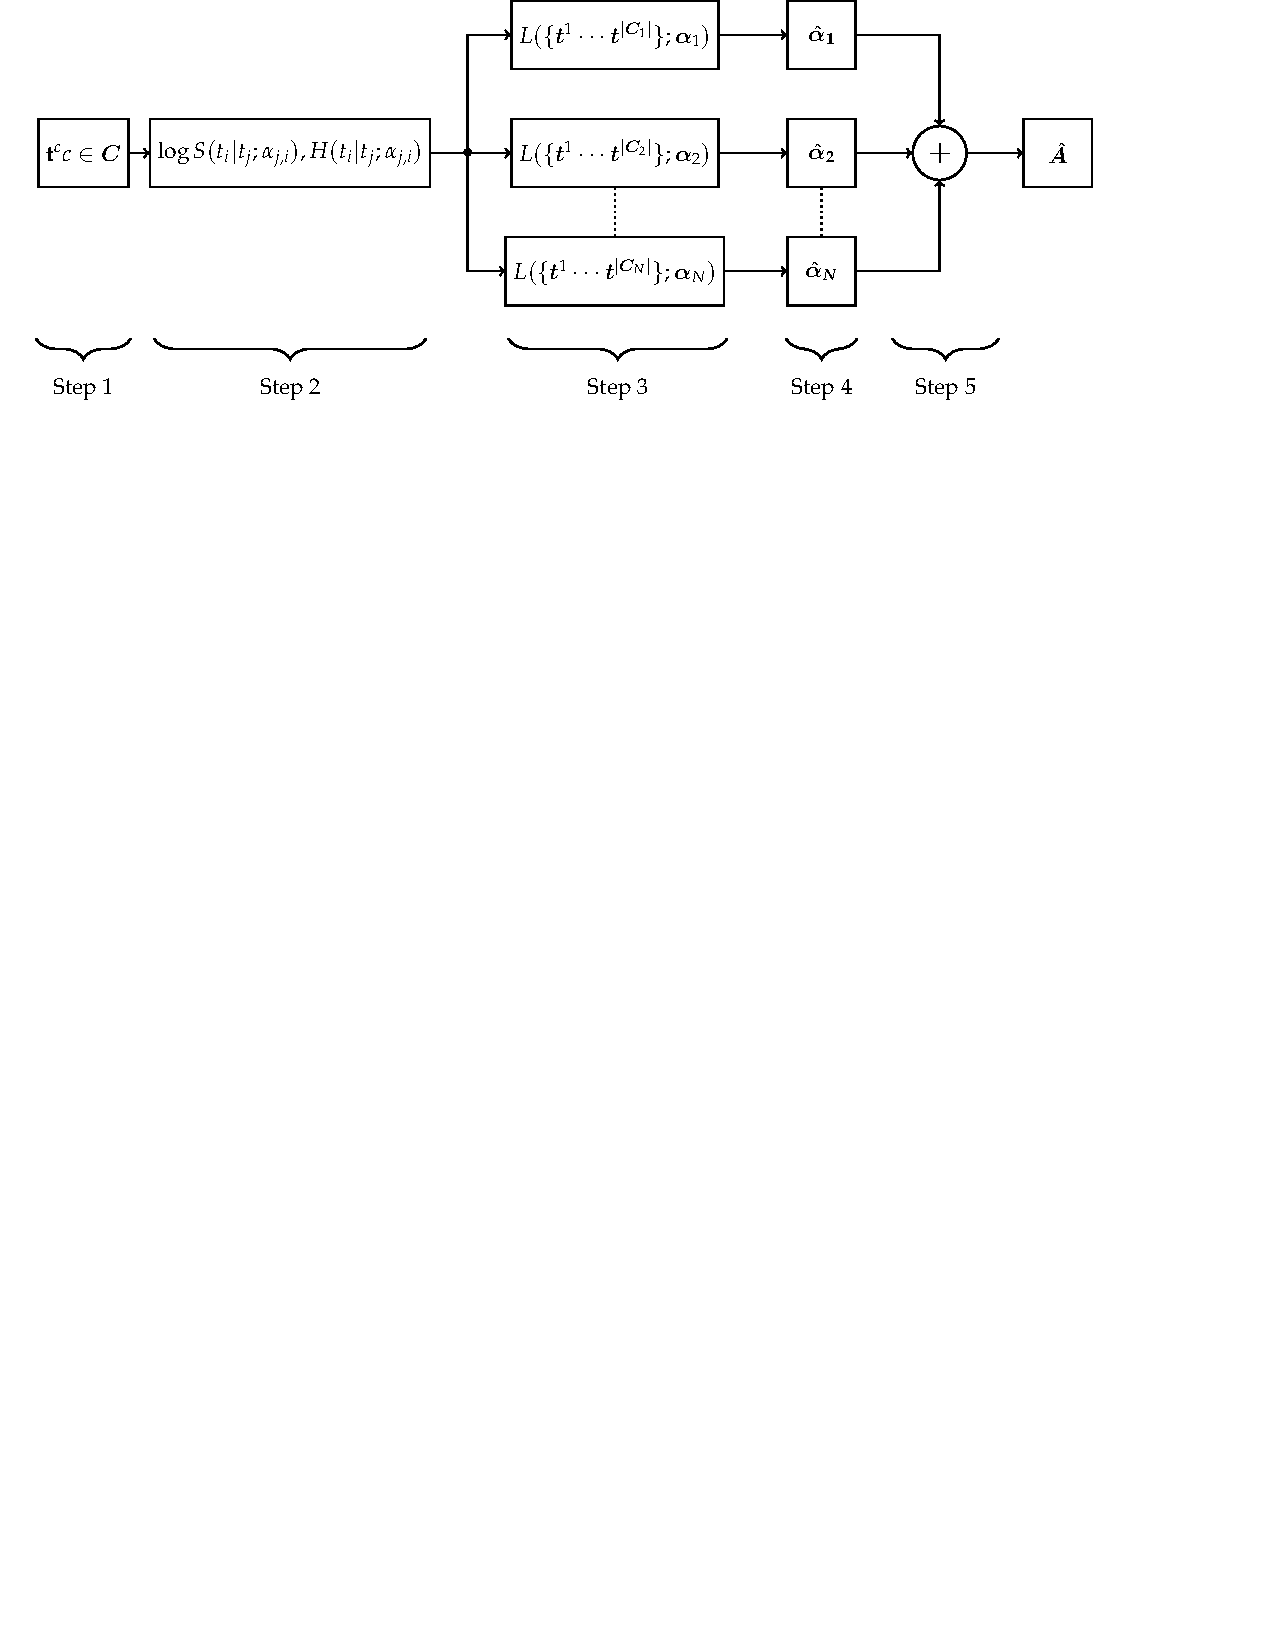
\includegraphics[trim={0 21cm 0 0}, width=\linewidth]{diagram_parallelization.pdf}
  \caption{Diagram of the NetRate parallelization process} 
	\label{fig:diagram_parallelization}
\end{figure}

Originally, the algorithm computed steps 3 and 4 sequentially. Once the transmission rates of a row of the adjacency matrix were computed, it continued with the following one. However, in a parallelized NetRate, they are all computed at the same time with step 5 also involving the stacking of each of the \(\bm{\hat{\alpha}}_{n}\) vectors to form the matrix \(\bm{\hat{A}}\).
The components in step 2 correspond to the ones seen in Eq.\ref{eq:solution_netrate} and whose solution is the assembled version of the one in step 3.\\

Once the structure of the algorithm is laid out, it still remains to plan how each of the jobs in steps 3 and 4 are will be assigned to the available processors. Not all the jobs take the same amount of time to be computed because they heavily depend on the number of cascades for their given node. As an illustration, a network of 10 neurons is simulated, and the number of cascades belonging to each node is shown in Eq.\ref{eq:num_cascades}. 

\begin{equation}
	\centering
	NoC = \{12, 21, 62, 166, 21, 67, 17, 30, 18, 81\}
	\label{eq:num_cascades}
\end{equation}

The mean of the distribution is 49 and the standard deviation 46. This means that the number of cascades differs significantly from node to node and that an appropriate way of distributing the jobs is required in order to keep all processors similarly busy. This is necessary because the whole algorithm will not finish until the last processor has estimated the weight parameters belonging to the last node. \\

Let \(M\) be the number of processors and \(N\) the number of nodes, where \(N > M\). The first \(M\) with the largest number of cascades are assigned in order to each of the processors. Each of the remaining \(N-M\) nodes is assigned to the processors following Eq.\ref{eq:argmin_processor}.

\begin{equation}
	\centering
	argmin_{n} \text{ } p_{i} + NoC_{n}, 
	\label{eq:argmin_processor}
\end{equation}

Where \(i \in [0,M]\) is the processor number, \(n \in [0, N - M]\) the node index and \(p_{i}\) is the sum of all the number of cascades assigned to processor \(i\). This method ensures that each of the processors has as close number of nodes as possible. Using Eq.\ref{eq:num_cascades} with \(N=10\), the distribution among \(M = 4\) processors becomes:

\begin{equation}
	\centering
	p_{1} = \{166\}, p_{2} = \{81, 21, 12\}, p_{3} = \{67, 21, 18\}, p_{4} = \{62, 30, 17\}
	\label{eq:distribution_processors}
\end{equation}

The resulting number of cascades for each of the processors becomes 166, 114, 106 and 109, respectively. This is a more balanced distribution than if the nodes had been assigned in any other way. \\

It remains to clarify in which order each of the nodes must be computed. One constraint that limits the algorithm is memory. The larger the number of cascades that need to be computed, the more memory is required for the algorithm to compute the weights. The relationship between the number of cascades and size of the network is exponential and, as it grows, NetRate makes use of a larger amount of memory. Each of the processors requires its own memory to perform NetRate in parallel. Thus, it becomes prohibitive to use several processors at the same time for large networks. However, some minor adjustments can be made to increase the capability of a parallelized NetRate by choosing which nodes are computed first. If all the largest nodes are computed at the same time the computer will not be able to finish the task for a sufficiently big network. For this reason, half of the processors will start with the nodes whose number of cascades is the lowest. The other half will do the opposite and compute the ones with the highest number of cascades. This way, the number of cascades computed at any given moment is levelled out and the likelihood of sudden spikes of memory usage are reduced. \\

As mentioned above, the CVX package cannot be parallelized naturally. Since the previous attempts to do so failed \cite{pranav_report}, a new method had to be implemented. For this project, instead of parallelizing NetRate from within MATLAB, several MATLAB instances are opened that work independently of each other. Each of these instances outputs a csv file and they are all combined by a Python script at the end of the computation. 

\subsection{Speed improvement results}

In this section the speed performance of the parallelized NetRate is evaluated. The computation time of NetRate for networks of different sizes, a stimulation period of 4000 ms and using 1, 4 and 8 processors is displayed in figure \ref{fig:speed_netrate}. Due to memory constraints of the computer, only up to 40 nodes were evaluated. As explained above, the more processors used at the time the more memory is required and this made the algorithm stall when using 8 processors in a network of 50 neurons.\\

\begin{figure}
\centering
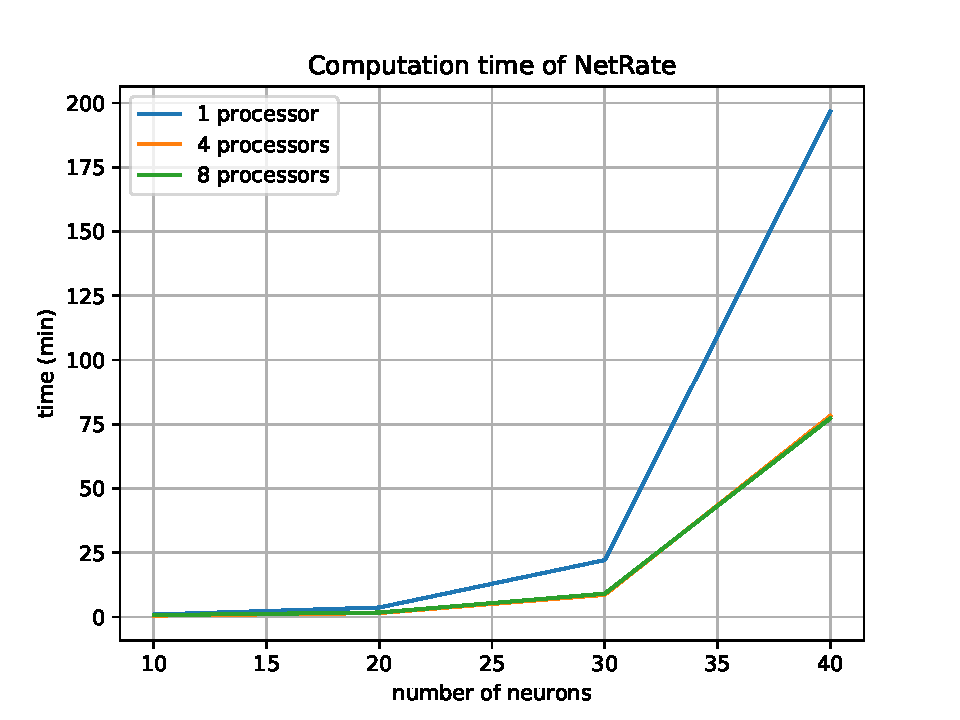
\includegraphics[width=0.8\linewidth]{computation_time_netrate.pdf}
\caption{Computation time of NetRate}
\label{fig:speed_netrate}
\end{figure}

There is a significant improvement in the speed of the algorithm when comparing 1 processor to 4 and 8 processors. For 30 neurons, it takes 22, 8 and 9 minutes for 1, 4 and 8 processors whereas for 40 neurons, it takes 196, 77 and 78 minutes. Although these are good results, they are far from ideal. 
Firstly, the time it takes to do the computation with 4 processors is not 4 times faster than with just one processor. It is, in fact, approximately 2.6 for the networks with 30 and 40 neurons. 
Moreover, using 8 processors instead of 4 results in no speed improvement for any of the networks. It is difficult to understand this behaviour because deeper analysis shows that all 8 processors are busy during the computation of the algorithm. One possible explanation is that the only steps that are actually being parallelized are number 3 from figure \ref{fig:diagram_parallelization}, where the optimization problem in \ref{eq:optimization_netrate} for each of the rows of the adjacency matrix is built, and half of step 4, where the CVX package is used but the solver has not been called. This means that the solver in the CVX package is a shared resource among all the running MATLAB instances and that each of the processors waits in a queue to compute its own row of the adjacency matrix. Further investigation into this hypothesis leads in this direction: when printing the progress of the optimization solver SDPT3, there is a linear behaviour i.e all processes print in an orderly fashion and there is no overlapping between them. However, further research into this issue must be carried out.\\

In this section it has been described what the steps of NetRate are, how the parallelization is implemented and what its limitations are. It is necessary to have a fast algorithm for it to be used with large networks. Finally, it was shown that although there is a significant improvement in the speed of NetRate, it is not as good as desired, and it also poses further restrictions on memory usage.  


\chapter{Simulating a biological neural network}

Up until now the inference of networks using NetRate has been used only on simulations. A random structure was generated and the spikes simulated using the Brian simulator. This is very useful because it allows the possibility of comparing the inferred network to a ground truth and evaluating the performance of the algorithm. However, the goal is to be able to implement NetRate on real biological networks whose topology could provide insight to scientists. The analysis of real biological neural networks is met with many difficulties that need to be dealt with.\\

The main problem regarding the inference of the connectivity of a biological neural network is the lack of a ground truth with which to compare the capabilities of the algorithm. Although never to a full extent, there are certain ways that can help deal with this issue. The first is to simulate a network that replicates the characteristics of the real one. Under the assumption that the simulated network has a similar behaviour (not necessarily same connections) to the biological one, the algorithm can be implemented and tested. Then, the accuracy obtained can be taken to be an approximation to the accuracy of the inferred real network. However, this is a very big assumption and in reality the simulated network might be very different to the real one. However, the main reason for testing on a simulated network is to verify that any change in the stimulation model of the system or any new method of cascade generation is still valid. A deeper explanation of this topic will be given in section \ref{sec:number_of_spikes}.\\

Another way of measuring performance would be to separate the dataset into training and testing and running NetRate on the training set. With the resulting estimated weights, given that a set of neurons have fired at time \(t\), estimate the neuron with highest probability of spiking. The relevance of this analysis stems from the fact that if \(\alpha_{j,i}\) is high, then the probability of neuron \(i\) spiking given that neuron \(j\) has fired is also high. If the accuracy of prediction is sufficiently high, the network can be taken to be correctly inferred.\\

It is important to find a suitable dataset to analyse. It must either be made out of voltage readings from an array of sensors in a cluster of neurons or spike times and indices\footnote{Here, the index is the neuron number that generates a specific spike}. The second option is preferable because it would not require spike sorting. It would also be advantageous if the dataset contained some biological information as to the type of neurons present in the system, how they are connected (if there is any biological way of measuring it) or where they are located. This information would help in creating a reliable simulation of the system and having a way of estimating a ground truth. In the next section, the dataset that is going to be used will be discussed. 

\section{Mouse somatosensory cortex neuron dataset}

For this project, the dataset that will be studied is the CRNCNS mouse somatosensory cortex SSC-3 dataset \cite{ito2016spontaneous, ito2014large, litke2004does}. This is a recording of the spiking activity from a mouse's somatosensory cortex brain cells. These cells were grown in cultures for 2-4 weeks and then measured with a 512 multi-electrode array that sensed the voltage in the culture for each of the neurons. These recordings were then spike sorted using PCA. \\

The somatosensory cortex is a set of modules located in the neocortex in the brain. The neocortex is vital in giving humans many of its cognitive abilities such as language processing, logic, sensory perception and many others. The neocortex shares many of its characteristics and architecture across different species of animals which makes it a very interesting subject of study. The somatosensory cortex is special because it is responsible for the touch sensations and because its anatomy and physiology has been intensively investigated \cite{markram2015reconstruction}.\\

The dataset consists of 25 different 1 hour recordings with a varying number of neurons ranging from 98 to 594. The average number of spikes per neuron for all datasets is 2.1 Hz and the sampling frequency is 20 kHz. The dataset also contains additional information on the x-y coordinates of each of the neurons in the cultures. With all this information, it is of interest to analyse what the distribution of spikes is. Neurons with larger connections will spike more often than the rest. Figure \ref{fig:histogram_spikes} displays how the spikes are distributed in the network. It is clear that the number of spikes per neuron follows an exponential distribution. Most of the neurons have sparse connections and will fire less than 6000 times during the length of the recordings while a few neurons will fire many times due to their high connectivity. In the next section, a simulated network will be implemented that tries to mimic the observable characteristics of the real 98 neuron network.\\

\begin{figure}[H]
	\centering
	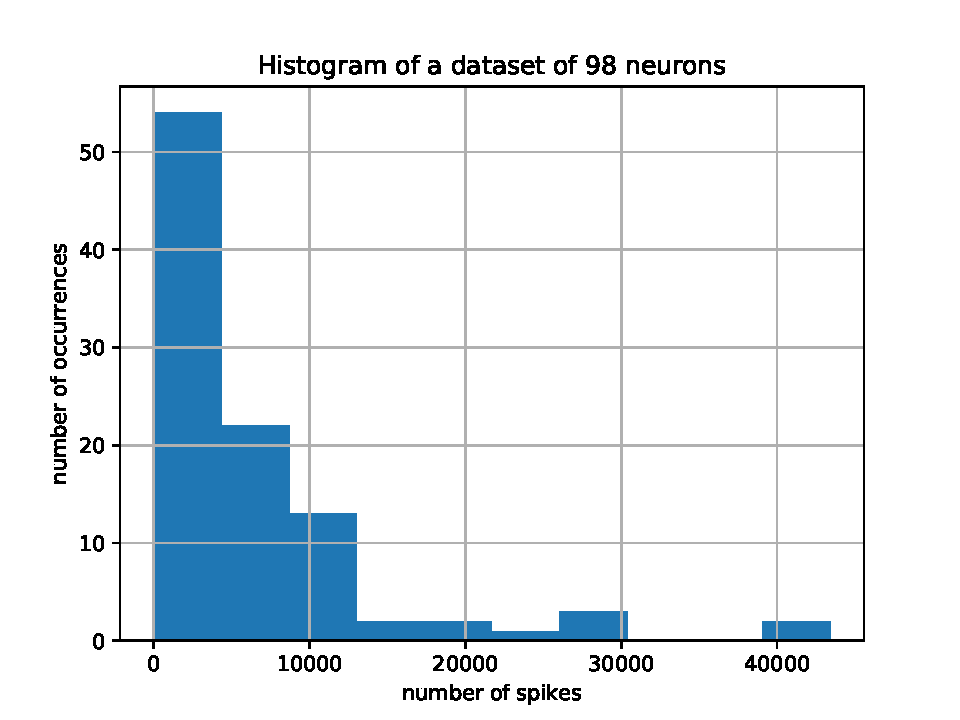
\includegraphics[width=0.8\textwidth]{histogram_number_spikes_dataset.pdf}
	\caption{Histogram of the number of spikes in a network of 98 neurons}
	\label{fig:histogram_spikes}
\end{figure}

\section{Input stimulus to the system}

Previous work \cite{alexandru2018estimating} simulated a network whose input was a DC voltage that stimulated each of the neurons one by one for a defined period of time (4 seconds). This proved to be very useful because it facilitated the analysis of each of the neurons regardless of their level of connectivity and because it provided a systematic way of generating cascades (more on this in section \ref{sec:simulating_cascade_generation}).
However, the neural system cultures from the dataset are not stimulated. Instead, they are left alone to interact between each other. The neurons then communicate independently of the outside environment and spike at a lower frequency as a result. \\

The input stimulus cannot be left unchanged because the behaviour of the network would be radically different to that of the real one. It cannot be null either because then no interactions between the neurons would occur. Some type of random input noise must be present in order to have spikes. Moreover, the new model should have biological significance since a real network is being replicated. An option is investigated that could potentially meet these requirements.\\

\subsection{System with random spikes}\label{sec:sys_rand_spikes}

The proposed model intends to mimic biological behaviour by assuming that neurons spike when they want to transmit some information that they have conveyed by themselves. In order to do so, a random neuron is selected from the network and stimulated with random noise for some length of time.
The benefit of this model arises from its ability to insure that every neuron has roughly the same probability of originating a spike train, from its random behaviour in the system and from its major biological resemblance than the model used in \cite{alexandru2018estimating}.\\

The noise that is input to the selected neuron is taken from the absolute value of a normal distribution of zero mean and standard deviation equal to \(\alpha\). Since, a model of only excitatory neurons is being implemented, negative values from the distribution are not valid. \\

The amount of time the selected neuron is stimulated for is also random. It is taken from a uniform distribution in the range 0 to 200 ms. There is no evidence to support the selection of this number since to this day, the behaviour of the neuron is not very well understood. However, it must be sufficiently large for the neuron to spike but to not too big so as to allow other neurons to be stimulated too. \\



\section{Number of spikes}\label{sec:number_of_spikes}

It can be seen in table \ref{tab:spike_characteristics} that one of the most obvious differences between the real dataset and the previous simulations is the total number of spikes. The number is significantly smaller than before even though the observation time is larger. This is because the stimulation model forced the neurons to spike very frequently. In \cite{alexandru2018estimating} the total observation time was equal to the defined length of stimulation multiplied by the number of neurons. Since the stimulation period was found to be optimal for 4 seconds, then for a network of 98 neurons, this would result in a total of 392 seconds of recordings. \\ 

\begin{table}[]
\centering
\begin{tabular}{|c|c|c|c|c|c|}
\hline
Type of network  & Neurons & Duration & Number of spikes & Mean    & Freq spikes/neuron \\ \hline
Real             & 98                & 3600 s           & 636878           & 6498.2  & 1.2 Hz               \\ \hline
Sim. DC stimulus & 98                & 392 s            & 4038313          & 41207.3 & 105.12 Hz            \\ \hline
\end{tabular}
\caption{Spike characteristics of different types of neural networks}
\label{tab:spike_characteristics}
\end{table}

On the other hand, the real dataset consists of recordings of one hour. Therefore, the model of the simulation must be such that the number of spikes is roughly the same for a 1 hour simulation length. This can be achieved by multiplying by varying the parameter \(\alpha\) from the input stimulus of the model. This variable controls the standard deviation of the absolute normal distribution defined in section \ref{sec:sys_rand_spikes}. The larger it is, the more voltage will be induced into the neuron and the higher its probability of spiking.
Every simulation will have a considerably different number of spikes given the parameter \(\alpha\). However, its effect on the number of spikes is investigated for a 1 hour simulated network of 98 neurons. This will give a rough estimate of what the parameter value should be. Figure \ref{fig:I_var_plot} shows that the most appropriate value of \(\alpha\) is 4. 

\begin{figure}[H]
	\centering
	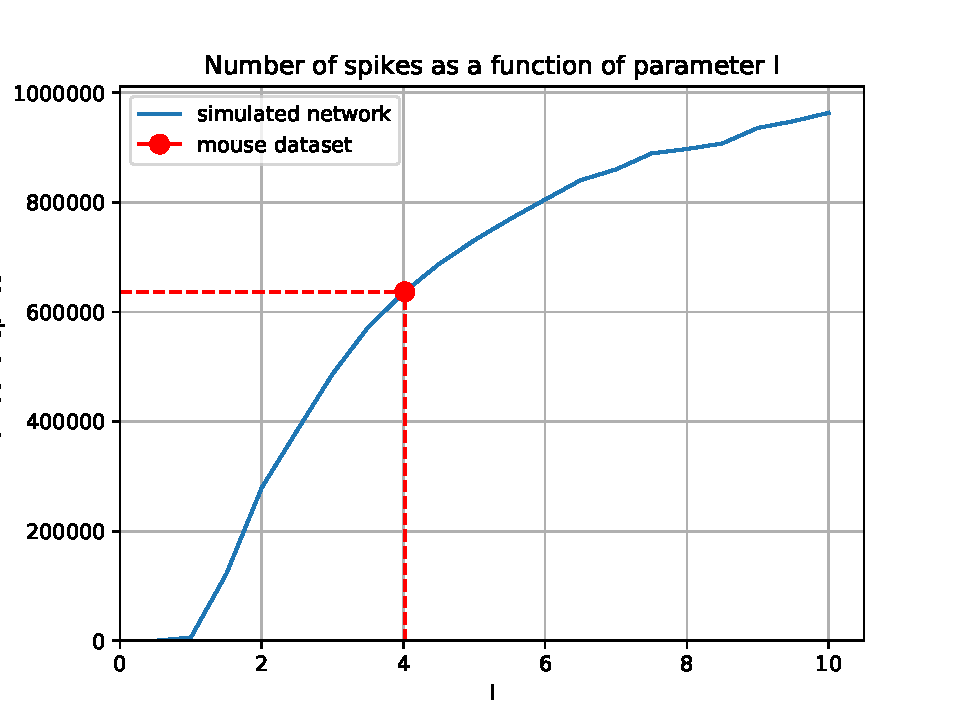
\includegraphics[width=0.8\textwidth]{I_var_plot.pdf}
	\caption{Number of spikes as a function of the parameter I for a 1 hour simulated network of 98 neurons and a random spike stimulus}
	\label{fig:I_var_plot}
\end{figure}


% Number of spikes
% 	I_var
% 	Frequency of spikes
% Shape of the histogram
% 	Changing the randomisation of the adjacency weights
% Types of neurons
% 	Excitatory and inhibitory
% 	What type of excitatory



\section{Cascade generation}\label{sec:simulating_cascade_generation}

Once the network model is defined what remains to clarify is how the cascades will be built. The method used in \cite{alexandru2018estimating} was simple and consistent. Since a DC stimulus was given to one neuron at a time, this neuron was selected to be the beginning of the cascade. This cascade would last for \(T\) length of time and only the first firing of each neuron would be taken into account. This insures that the third assumption from \cite{rodriguez2011uncovering} is not broken, i.e observable artefacts in are binary. Moreover, with this cascade generation method, cascade independence was guaranteed because it provided a clear entry point into the diffusion process. Since the system no longer has a DC input, the cascade generation method must be changed. When selecting an appropriate method of cascade generation, certain factors are taken into account.
\begin{enumerate}
\item The higher the number of cascades that are generated, the more information will be conveyed and, in general, the better NetRate will be able to infer the connectivity of the network. 
\item The more separated the cascades are from each other in the time domain, the more independent they will be. Although in \cite{rodriguez2011uncovering}, independence is defined as uniqueness of spikes for all the cascades in the diffusion process, it will be redefined as the likelihood of the spikes in the time horizon being caused by a previous spike in the same cascade. This means that not only all spikes are unique within all the cascades but that, there is no influence from the previous cascades on the present one.
\item A high sparsity insures that enough cascade information is obtained from all the neurons in the network. Otherwise, only neurons who spike often will be the ones generating cascades.
\end{enumerate}

\subsection{Method of maximum cascades}

One way of building cascades is the proposed method of maximum cascades. This is a very simple approach that uses the first spiking neuron as the beginning of the cascade. This cascade lasts for the defined horizon and includes all the firing activity within this time period. This process is repeated after the last spike of the generated cascade and until the whole time series has been evaluated. It is worth remembering that, in the case of one neuron firing twice within the same time period, only the first one is taken into account and recorded in the cascade. As an example, let there be a network of 5 neurons that spike during a recording of 12 seconds and let the firing times and neuron indices be:

\begin{align}
	\centering
	firings = &\{1.5, 2.6, 4.7, 8.1, 8.4, 9.4, 11.2\}\\
	indices = &\{4,  3,  5,  3,  2,  2, 4\}
\end{align}

Then, using the method of maximum cascades, the resulting two cascades would be the ones seen below:

\begin{align}
	\centering
	\textbf{t}^{1} = &\{\infty, \infty, 1.1, 0, 3.2 \}\\
	\textbf{t}^{2} = &\{\infty, 0.3, 0, 2.1, \infty \}
\end{align}

The first cascade starts at time \(t=1.5s\) and ends at \(t=6.5s\). During this time, neurons 3, 4 and 5 spike. Then, the second cascade, starts at time \(t=8.4s\) and finishes at \(t=12s\). Here, neurons 2, 3 and 4 spike. However, although neuron 2 spikes twice, only the first firing is taken into account. It is also worth remembering that, cascades are based on time differences rather than absolute times. \\

The advantage of this method stems from the large number of cascades that are generated. Every spike is used for generating cascades and, thus, the number of cascades is maximized. However, this is done irrespective of their quality. The quality of a cascade is defined as the fidelity of the probabilistic description of the network. In other words, how well it represents the true nature of the system. As an example, let the firings and indices of a simulation of 20 seconds with a horizon of 10 seconds be the ones in \ref{eq:quality_cascades} and let the network connections be the ones in table \ref{tab:quality_cascades}.

\begin{align}
	\centering
	firings = &\{1, 9, 11, 12, 19\}\\
	indices = &\{1, 2,  3,  4, 2\}
	\label{eq:quality_cascades}
\end{align}

The resulting cascades would then be:

\begin{align}
	\centering
	\textbf{t}^{1} = &\{0, 8, \infty, \infty \}\\
	\textbf{t}^{2} = &\{\infty, 8, 0, 1 \}
\end{align}

Although the above cascades are well constructed, the second cascade is of poor quality. This is because, under a deterministic model where there is no noise, the cascade would lead to believe that there is a connection between nodes 3 and 4 when, in fact, the spiking of node 4 was caused by either node 1 or 2. Since NetRate is made for inferring networks under stochastic conditions, this scenario could happen under an otherwise perfect system. However, the cascade method of maximum cascades is fundamentally flawed because cascades are not independent. The diffusion process from the first cascade has not reached a steady state and it has affected the second cascade. A new cascade method is proposed where the independence of cascades is increased. 

\begin{table}[H]
\centering
\begin{tabular}{|c|c|}
\hline
Source & Target \\ \hline
1      & 2      \\ \hline
1      & 4      \\ \hline
2      & 3      \\ \hline
2      & 4      \\ \hline
3      & 2      \\ \hline
\end{tabular}
\caption{Network connections example}
\label{tab:quality_cascades}
\end{table}


\subsection{Method of optimal independence}

Under the new definition, independence of cascades cannot be guaranteed. Any spike that occurs could cause another neuron to become unstable in the future or could, at least, contribute to this happening by increasing its membrane potential. However, it can be improved significantly by allowing the network to reach a steady state before starting the cascade.\\

The method of optimal independence poses a stability constraint on cascade generation. This is achieved by requiring the first spike of each cascade to be a specific amount of time far away from its immediate previous spike. For simplicity, in this project, this time variable will be equal to the time horizon.\\

This method increases the quality of the cascades in comparison to the one of maximum cascades. However, since it is more difficult to generate cascades that meet the requirements, there will also be fewer cascades. This is not always a problem, since, many times the number of cascades generated by the first method exceeds the computation capabilities of the computer at hand. By modifying the stability period parameter, the number of desired cascades can be chosen and only the ones with the highest independence will be used.

\section{Concluding remarks}

At the beginning of this chapter the need for a simulated network that approximated the biological one was explained. Such a model can provide an approximation of performance of the algorithm. It is based on the assumption that the simulation is a faithful representation of the real nature of the network. Moreover, the differences between previous simulated networks and this new real network make it vital to verify that the algorithm would still work under these new conditions. \\

A new model was defined that tries to mimic the behaviour of the real mouse recordings. For this reason, instead of simulating a network whose input consisted of a DC stimulus, a random input was established that consisted of the absolute value from a normal distribution of mean zero and standard deviation \(\alpha\). This stimulus would be given for a random amount time to a random neuron in the system. \\

Finally, a new method of cascade generation was defined. This was necessary because the change of input stimulus made the previous approach obsolete. Following this new method, the number of cascades is maximized regardless of the quality of the cascades.









\chapter{Inferring the connectivity of a mouse's neuronal system}

In chapter 4 a neural network model was simulated to try and mimic the behaviour of the real network described in \ref{sec:mouse_dataset}. A new input stimulus and two cascade generation methods were proposed. In this chapter, the suitability of these new methods will be proved by inferring the connectivity of the new simulation model outlined in section \ref{sec:input_stimulus}. Moreover, the effect of the simulation duration and the network size on the performance of the algorithm will be assessed.\\

Once the suitability has been demonstrated, the same algorithm will be used to infer the connectivity of one of the networks from the CRCNS dataset. Further analysis of this structure will be carried out and its main characteristics will be described.\\

In order to evaluate the performance of the algorithm, the four metrics described in \ref{sec:performance_metrics} will be used. However, as outlined in \cite{pranav_report}, the structure of the network can have a great effect on NetRate's ability to estimate it. For this reason, for validating the suitability of the model, an average of 4 experiments will be used as the results displayed in this chapter.

\section{Proof of the suitability of the algorithm}\label{sec:proof_suitability}


\section{Effect of the size of the network and simulation time on the performance of NetRate}

It is of interest to analyse how the performance of the algorithm varies with different simulation times. Figure \ref{fig:results_10_neurons} shows the results for this analysis. It can be observed that the larger the simulation time, the better NetRate's ability to infer the network. This finding is to be expected due to the fact that the longer the observation length, the more information is captured. However, this behaviour begins to plateau after 1250 seconds of simulation time.\\

\begin{figure}
	\centering
	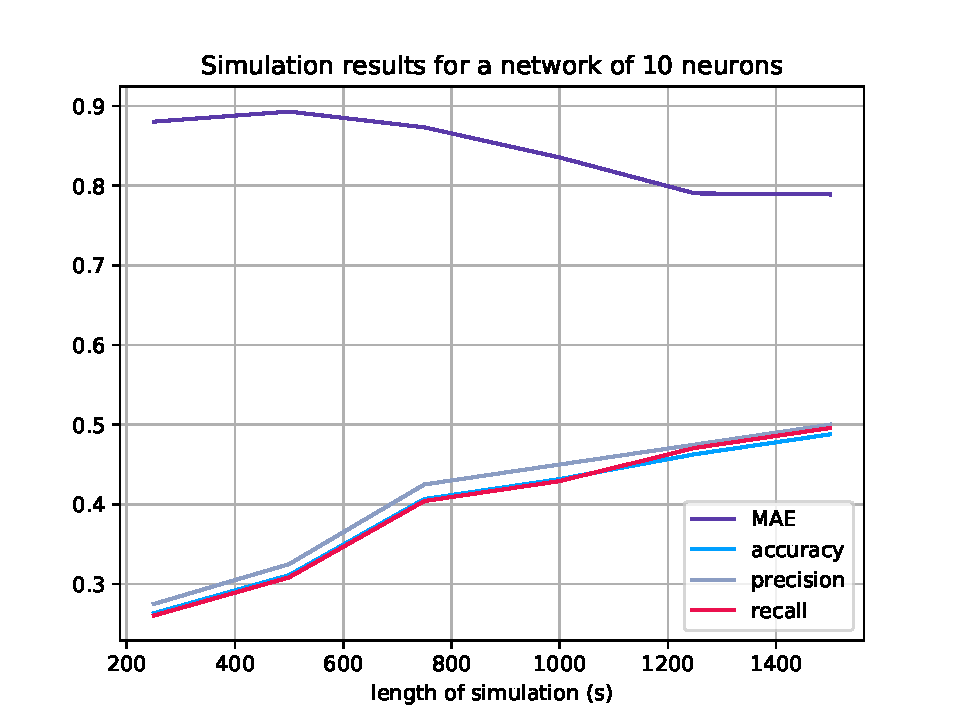
\includegraphics[width=0.8\linewidth]{results_10_neurons.pdf}
	\caption{Network inference performance for a neural network of 10 neurons}
	\label{fig:results_10_neurons}
\end{figure}




\begin{figure}
	\centering
	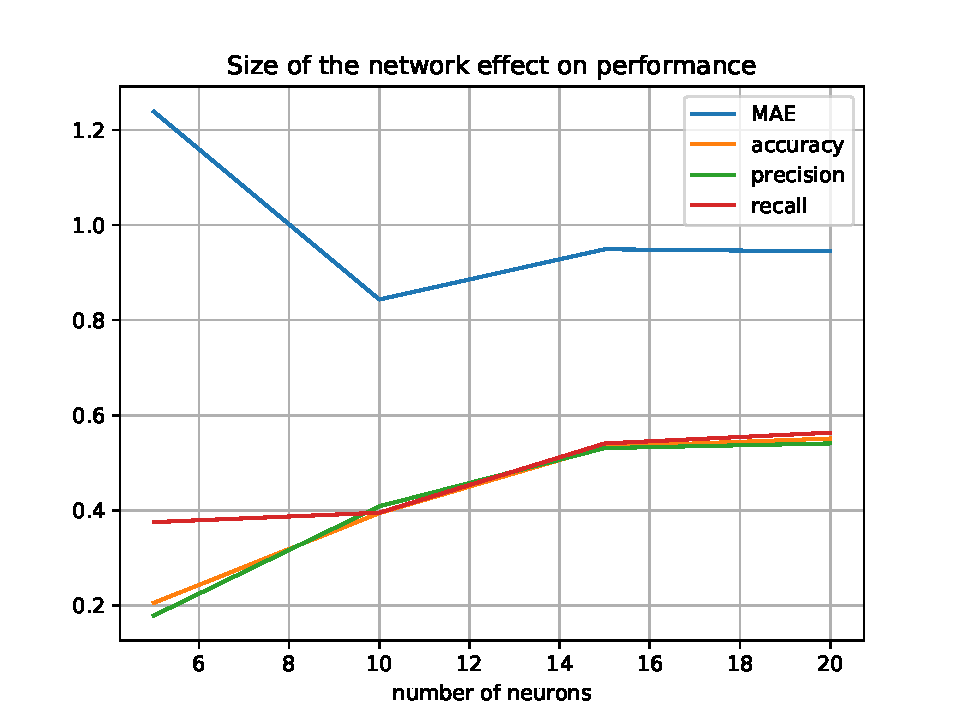
\includegraphics[width=0.8\linewidth]{size_effect_performance.pdf}
	\caption{Average network inference performance for different network sizes}
	\label{fig:results_network_sizes}
\end{figure}

\section{Evaluating the performance without a ground truth}
\section{Inference results}

Once the suitability of the algorithm has been proven, the connectivity of a biological neural network can be inferred. In this section, the 98 neuron network analysed in section \ref{sec:mouse_dataset} and whose evaluation suitability was proven in \ref{sec:proof_suitability} is the one evaluated. Due to the dataset being large enough, the \textit{optimal independence} method of cascade generation is employed. As explained in section \ref{sec:optimal_independence}, this will achieve a higher quality set of cascades.\\

When computing NetRate for a large dataset like the one at hand, the main constraint that the researcher has to deal with is memory. This is directly proportional to the number of cascades computed at any given moment. Therefore, if only one processor is being used, the constraint will be set by the node with the maximum number of cascades. For the current dataset and, using the \textit{optimal independence} method of cascade generation, this corresponds to neuron 12 with 7956 cascades. The computation of this node requires an array of size 18Gb but, with the resources at hand, such an operation is not possible. For this reason, the dataset is partitioned into a smaller set containing the first half of the spike recordings. If the system is assumed to be static\footnote{A network is static if no connections are created or erased during the period of observation.} for the whole length of the recording, then only the performance of NetRate could be affected by this split. The resulting maximum number of cascades is reduced to 5168, with the amount of memory required being lowered to 11Gb.\\

In figure \ref{fig:crcns_4_network}, the resulting inferred network is displayed. Each of the nodes is represented by a circle whose connections are the lines adjacent to them. Since the network is directed, the edges are represented by arrows that indicate the source and target of the connections. Each of the nodes in the figure is coloured according to their degree. Nodes in directed networks can be described by their indegree and outdegree i.e., number of inward and outward connections, respectively. Red nodes have more inward connections and blue nodes more outward connections. If their inward and outward degree is the same, in the figure, these cancel out and their colour becomes purple, just like neurons that have no connections at all. \\

\begin{figure}
	\centering
	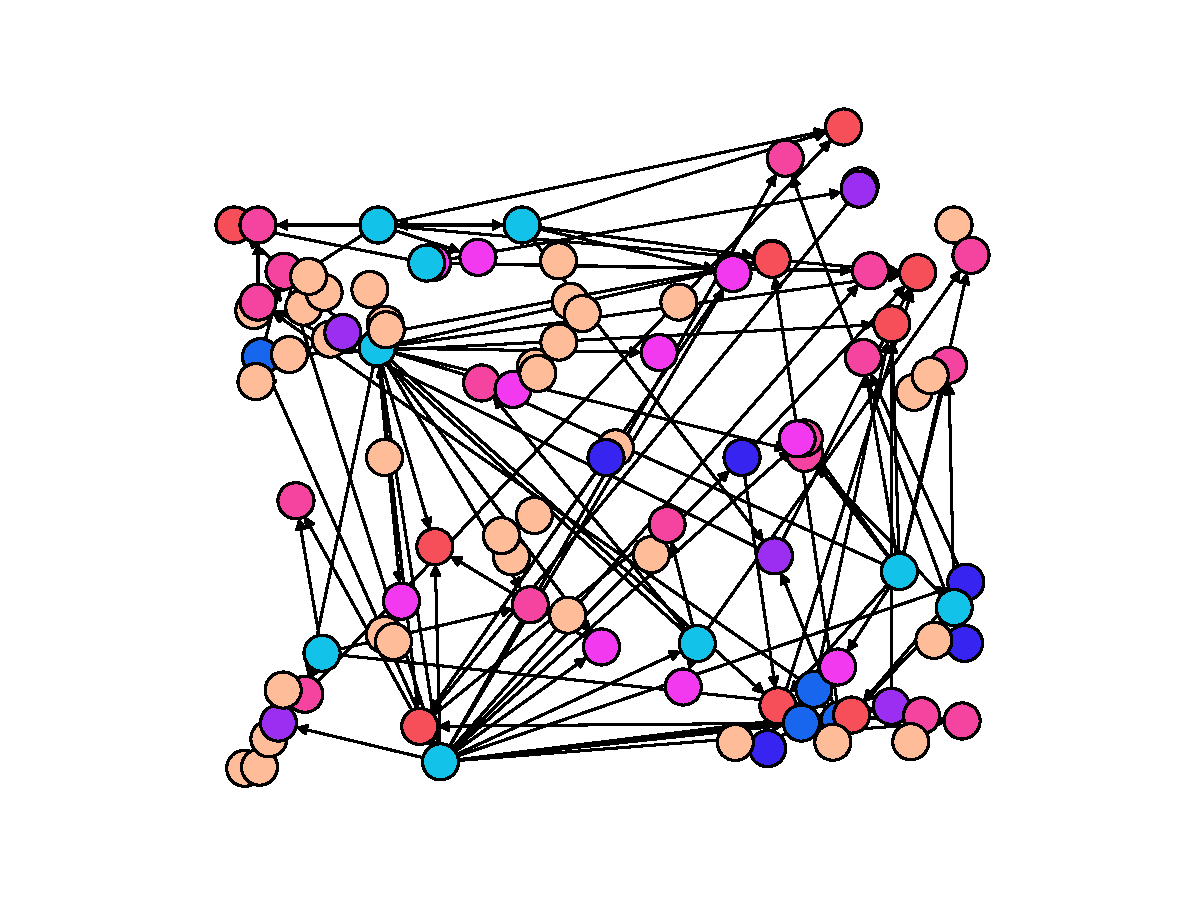
\includegraphics[width=0.8\linewidth]{crcns_4_50_xy.pdf}
	\caption{Inference of a biological neural network of 98 neurons. Red for indegree > outdegree, blue for outdegree > indegree and peach for non connected neurons.}
	\label{fig:crcns_4_network}
\end{figure}

\begin{figure}
	\centering
	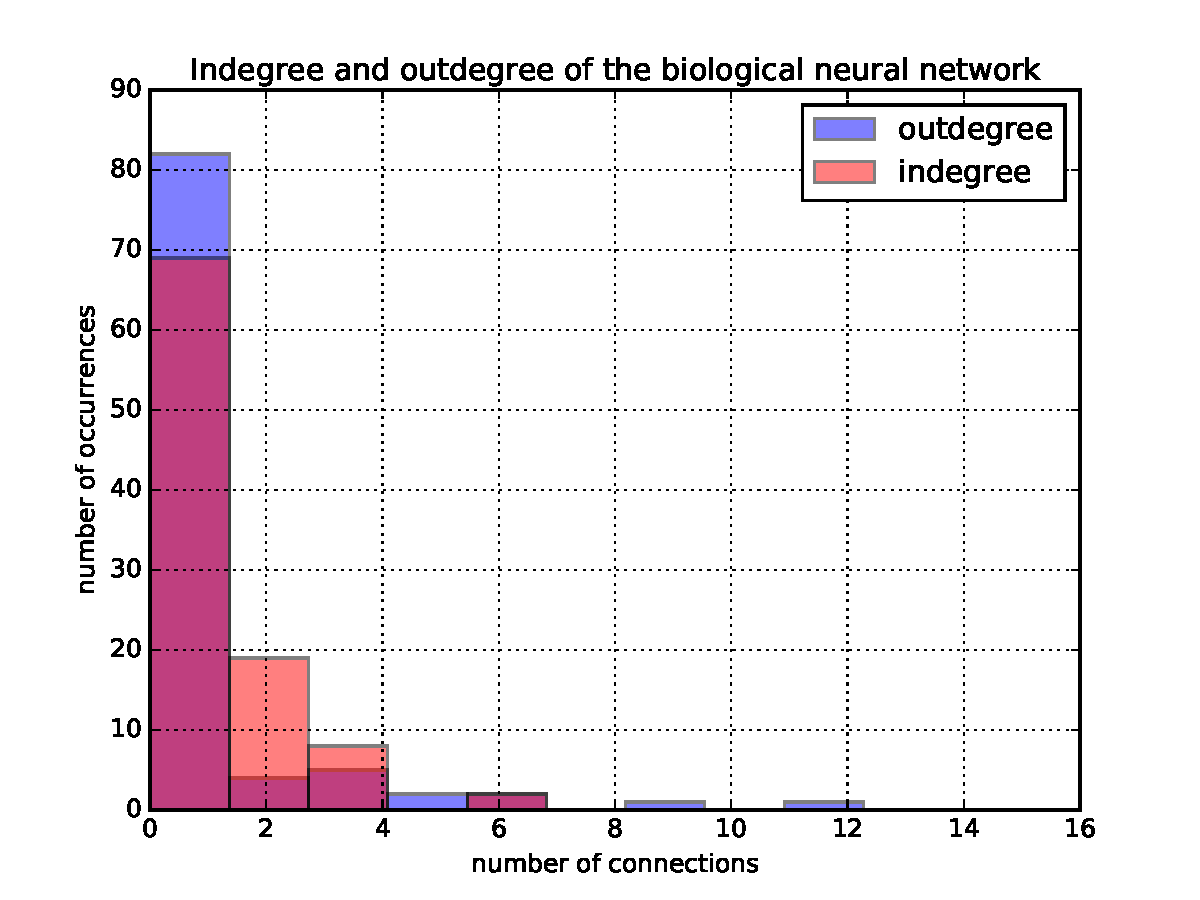
\includegraphics[width=0.8\linewidth]{degree_histogram_real_network.pdf}
	\caption{Indegree and outdegree histogram of a biological neural network}
	\label{fig:degree_histogram}
\end{figure}

An illustration of the degree of nodes in the network is shown in figure \ref{fig:degree_histogram}. As it can be observed, the degree distribution follows an exponential behaviour. Most of the nodes have at least one connection and very few have more. In general, neurons with a greater indegree will spike more often since they are more influenced by their neighbours. This finding agrees with the behaviour of spiking activity shown in figure \ref{fig:histogram_spikes}, where most neurons spike unfrequently and only few have a more intense spiking activity.\\

It is also of interest to analyse whether there exists any dependence between node distance and connectivity. In other words, whether two neurons close to each other have a higher chance of being connected. First, in order to test this hypothesis, the average distance between neurons is calculated. Since the dataset contains the x-y coordinates of all the neurons in the network, it is easy to see that this is equal to 831.57 \(\mu m\). Next, the average edge distance is computed. The value of this calculation is found to be 698.37 \(\mu m\). Although this value is lower than that of the average node distance, the difference is not sufficiently large so as to prove the validity of the hypothesis.









\input{evaluation/evaluation.tex}

\chapter{Software Package}

\section{Programming languages}

The software that is used for this project is based on a set of scripts written in bash, Python and Matlab. Each of these languages is used in a different where they excel due to either availability of libraries or ease of use. \\

Bash scripts are used as entry point to the software package
 

\section{System requirements}
\section{Folder architecture}
\section{Usage}


\chapter{Conclusion and future work}

\section{Summary of achievements}

The objective of this project was to improve the state of the art of neural network inference by increasing NetRate's performance or scalability. It was also intended for this algorithm to be used for the network inference of a biological neural networks. This objective brought along many challenges that had to be dealt with beforehand such as changing the network model and updating the cascade generation method. Overall, this project has been successful at achieving the defined goals. \\

\begin{enumerate}
\item In chapter 1, a brief explanation of the project was given. It also included what the objectives were. 
\item Chapter 2 explained the mathematical background behind the network inference algorithm and the previous work done in this area.
\item Chapter 3 explained how a novel method could achieve a certain level of parallelization in NetRate and increase the speed of the algorithm.
\item In chapter 4, the model for a biological neural network that mimicked a real biological one was devised. Moreover, two new cascade generation methods were proposed in order to adapt to the changes in the network model.
\item A new performance metric was proposed in chapter 5 for networks without a ground truth. Its drawbacks were analysed and illustrative results were shown.
\item In chapter 6 the suitability of the changes in the algorithm done in chapter 4 is proved. Then a biological neural network is inferred and its characteristics are analysed. Moreover, the performance metric outlined in chapter 5 is used to test the knowledge of the network. It was shown that NetRate is able to capture some network information from the real data.
\item Finally, in chapter 7, the software package used for this project is described. Moreover, the folder structure within which all the results are saved is explained.
\end{enumerate}

\section{Future work}

\subsection{Test on more recordings}

In this project, only recording 4 from the 25 available was used. This was due to the fact that it was the dataset with the lowest number of neurons. An extension of this project could investigate the structure of the rest of recordings in the dataset. 

\subsection{Increase the complexity of the network model}

The model of the network employed in this project consisted of only excitatory neurons. However, biological neural networks consist of many different kinds of neurons. Future work could study the effect of having inhibitory neurons in the system but inferring the connectivity of the network with the assumption of them all being excitatory. 

\subsection{Random spiking cluster model}

The network model used in this project was the random spikes model. This was a very simple introductory method to mimicking biological neural networks. However, a more complex model could be studied where clusters of neurons spike at random times. Otherwise, due to the large differences yet to be solved between the real recordings and simulated network readings, more parameters can be changed so that the similarity is increased.

\subsection{Update the spiking prediction metric}

A method for evaluating the performance of NetRate on networks without a ground truth was proposed and tested in chapter 5. This is a very simple metric, however, it fails to make the best predictions possible. For this reason, an update to this metric could be proposed where not only the first neuron to spike is given, but also all the previous spikes in the recording. With such information it could be possible to estimate the membrane potential of all the neurons in the network and obtain a higher prediction score.


\input{appendix/appendix.tex}

\printbibliography 
% \bibliographystyle{unsrt}
% \bibliography{bibs/sample}
% \addcontentsline{toc}{chapter}{Bibliography}

\end{document}
